\section{Versuchsbeschreibung}
\subsection{Versuchsaufbau}
Der Versuchsaufbau besteht aus einer Lampe die hinter einer verstellbaren 
Spaltblende montiert wird. Vor die Spaltblende wird eine Halterung für 
Farbfilter und eine Sammellinse montiert. Als letztes Bauteil auf der 
Optischen Bank wird ein Podest benötigt auf welches während der 
Versuchsdurchführung Prismen gestellt werden können. Vor das Podest wird 
nun ein Schirm mit einer montierten Skala aufgebaut. Das Podest hat eine 
Entfernung von 38,5 cm zum Schirm.
\begin{figure}[!htb]
\centering
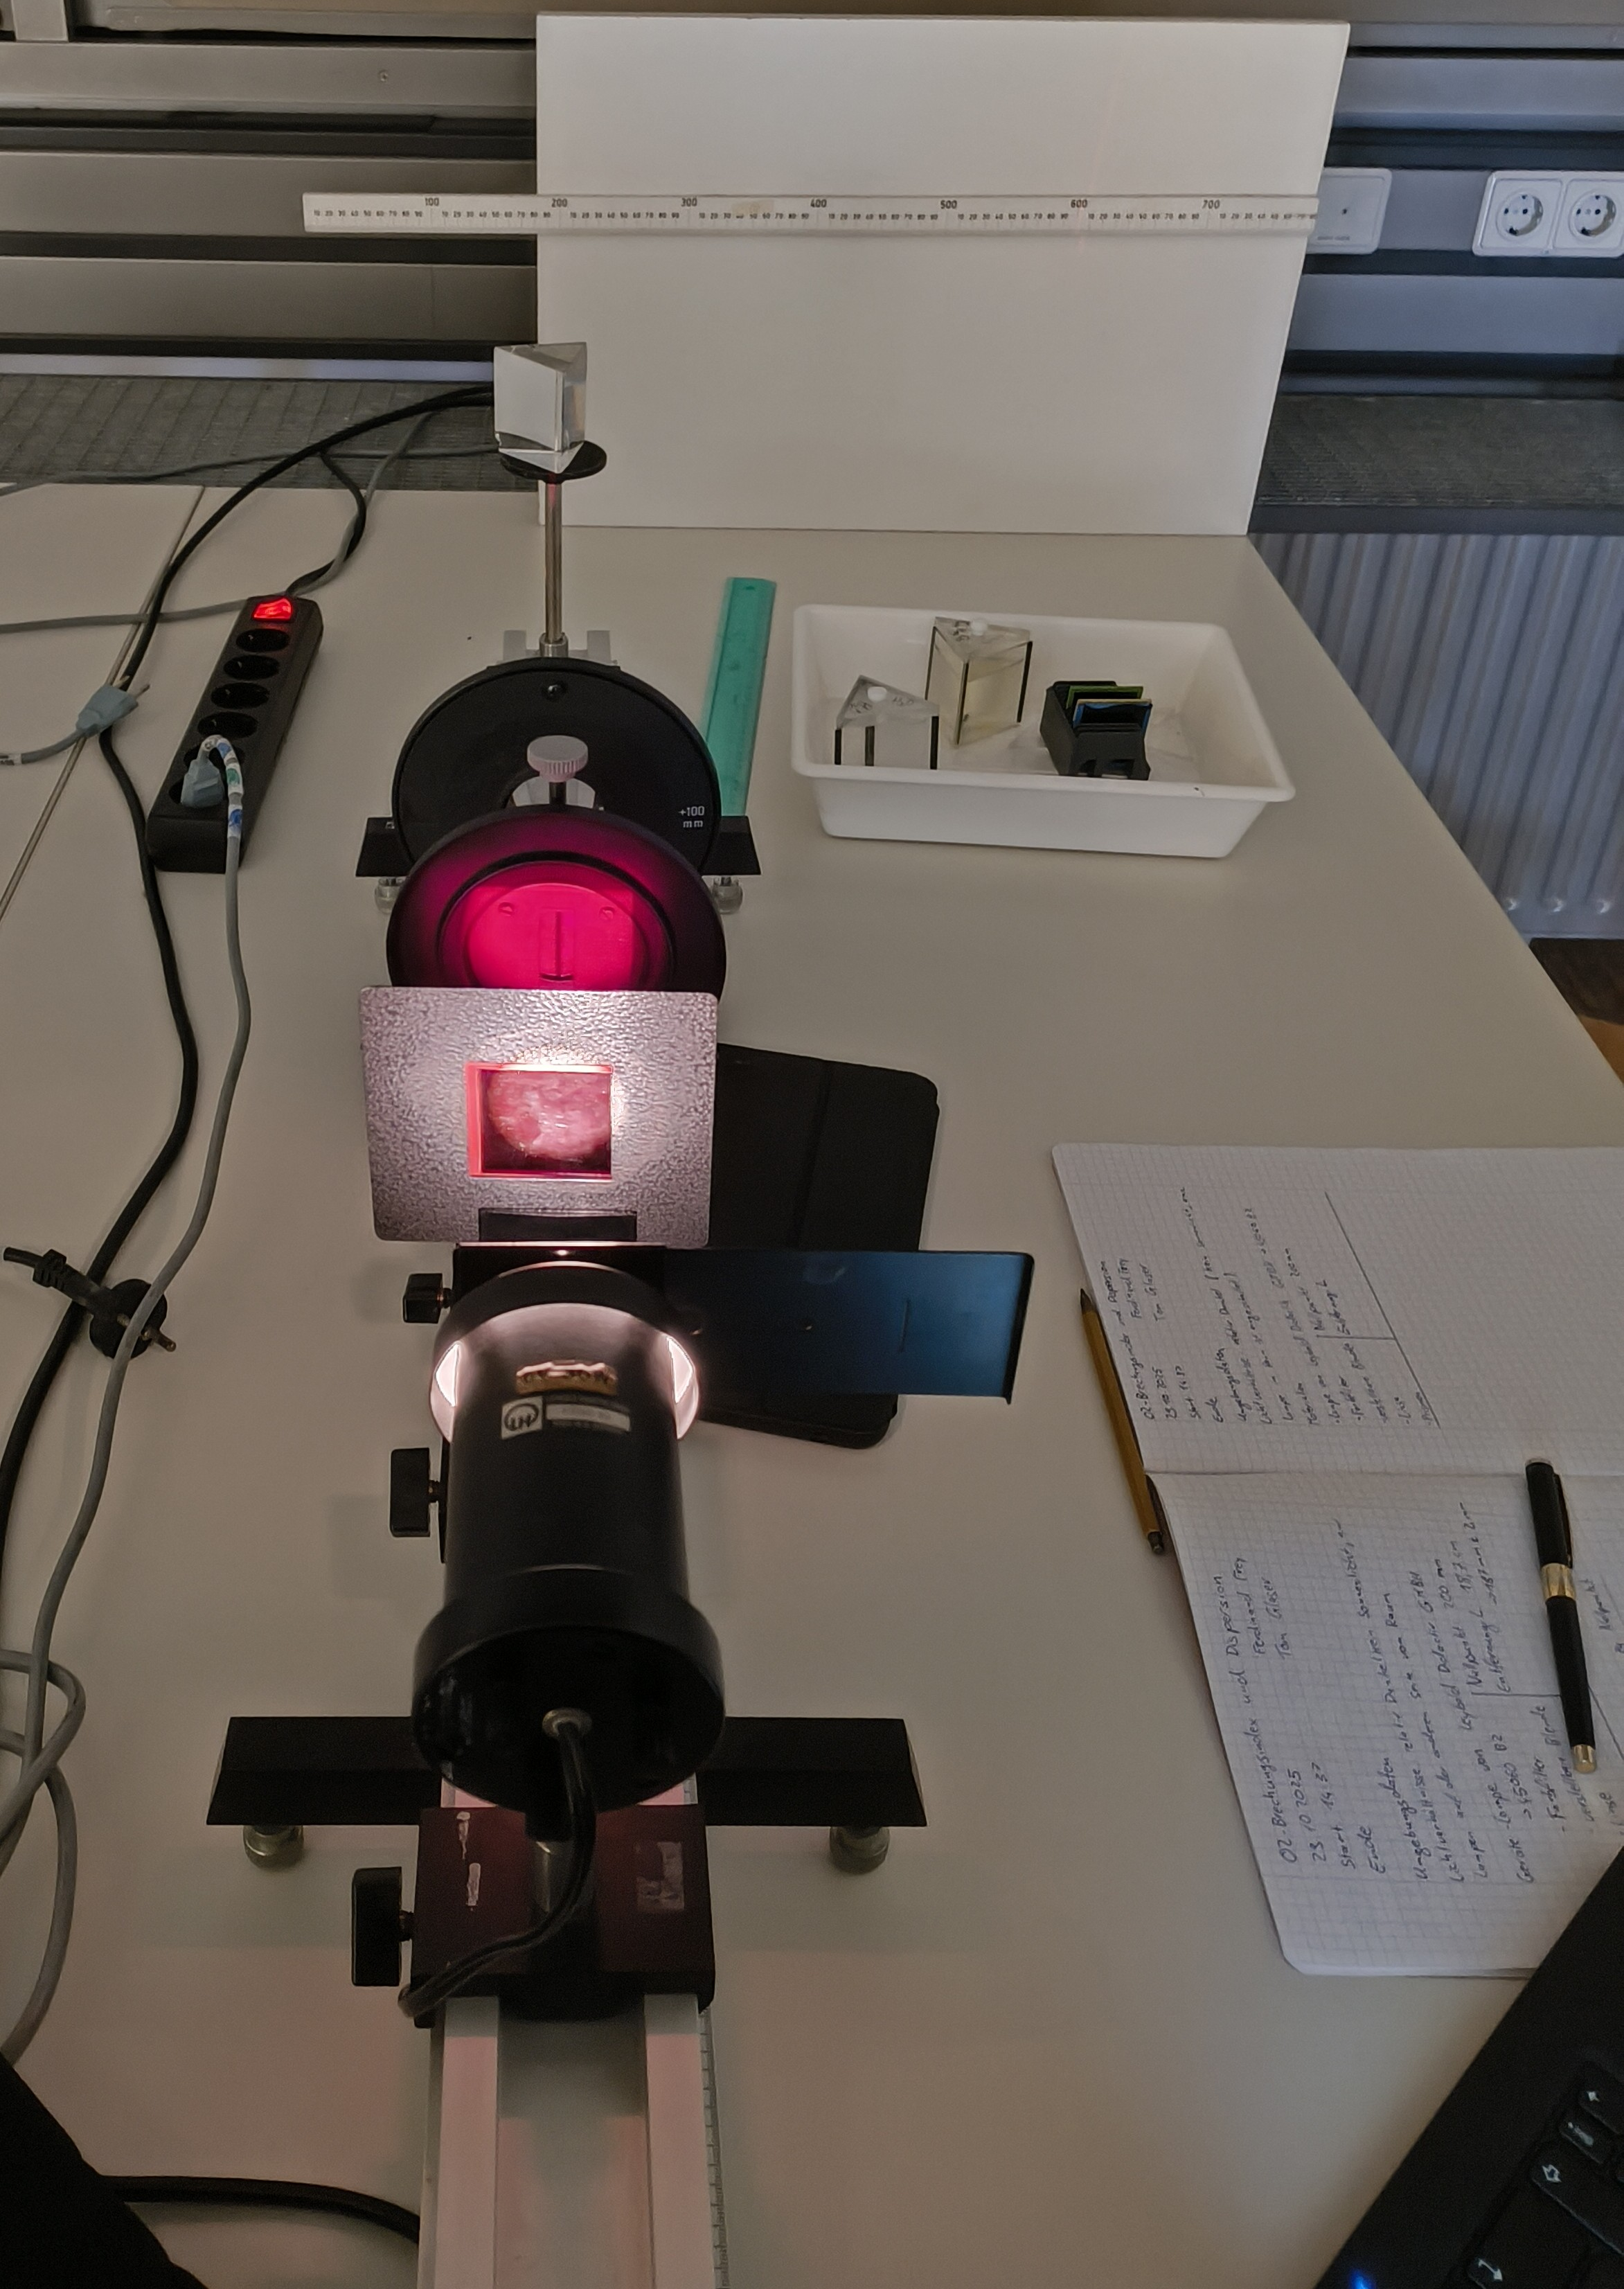
\includegraphics[scale=0.08]{Bilder/Richtiger Aufbau.jpg}
\caption{Ein Bild vom Versuchsaufbau, von vorne nach hinten. Lampe, Spaltblende, Farbfilterhalterung, Sammellinse, Podest und Schirm.}
\end{figure}


\subsection{Versuchsdurchführung}
Nun zur Versuchsdurchführung, zuerst wird die Lampe eingeschaltet und m
ithilfe der Spaltblende und der Sammellinse auf dem Schirm fokussiert, 
nun wird der fokussierte Punkt als $X_0$ vermerkt und die entfernung 
des Podest zum Schirm gemessen. Sobald diese Sachen erledigt sind kann 
mit der Durchführung richtig angefangen werden. Für den ersten Teil der 
Messung werden die zwei Vollprismen verwendet. Dazu wird das erste 
Prisma auf das Podest in den Lichtstrahl gestellt und solange vorsichtig 
gedreht bis das entstehende Farbspektrum nicht mehr weiter in Richtung 
des Punktes $X_0$ wandert. Nun werden nacheinander die Farbfilter in 
die Farbfilter Halterung gesteckt um die genaue Messung der verschiedenen 
Farben zu vereinfachen, denn jetzt wird die entfernung der jeweiligen 
Farblinie zu dem Punkt $X_0$ ermittelt. Sobald dies für alle Farbfilter 
durchgeführt wurde, werden die beiden Prismen getauscht und der ganze 
Vorgang wird wiederholt. Der zweite Teil des Experiment läuft analog zum 
ersten Teil des Experiments ab, doch jetzt werden nicht die Volprismen 
verwendet sondern die Hohlprismen die mit Flüssigkeit gefüllt sind. 